\documentclass{article}
\usepackage[letterpaper, left=2.5cm, right=2.5cm, top=2.5cm, bottom=2.5cm]{geometry}
\usepackage{graphicx}
\usepackage{epstopdf}
\usepackage{fge}
\begin{document}

\title{PAL Compiler Documentation }
\date{\today}
\author{Chris Pavlicek, Connor Moreside, Mike Armstrong, and Steve Jahns}
\maketitle

% From checkpoint 1 spec:
%
% Documentation
%
% Your documentation should describe what your group has done on the
% project. This does not mean that you should reiterate class notes; I want to
% know what is different about your group. Some things you may want to discuss
% include: handling of lexical units, syntax error reporting strategies, syntax
% error recovery (if any) , problems encountered and their solutions, etc.
% When writing, remember who is going to read it—skip the preli minaries
% and get to the point. There is a page limit of 12 double-spaced pages,
% not in cluding diagrams.

\section*{Overview}

\begin{figure}[h!]
\centering 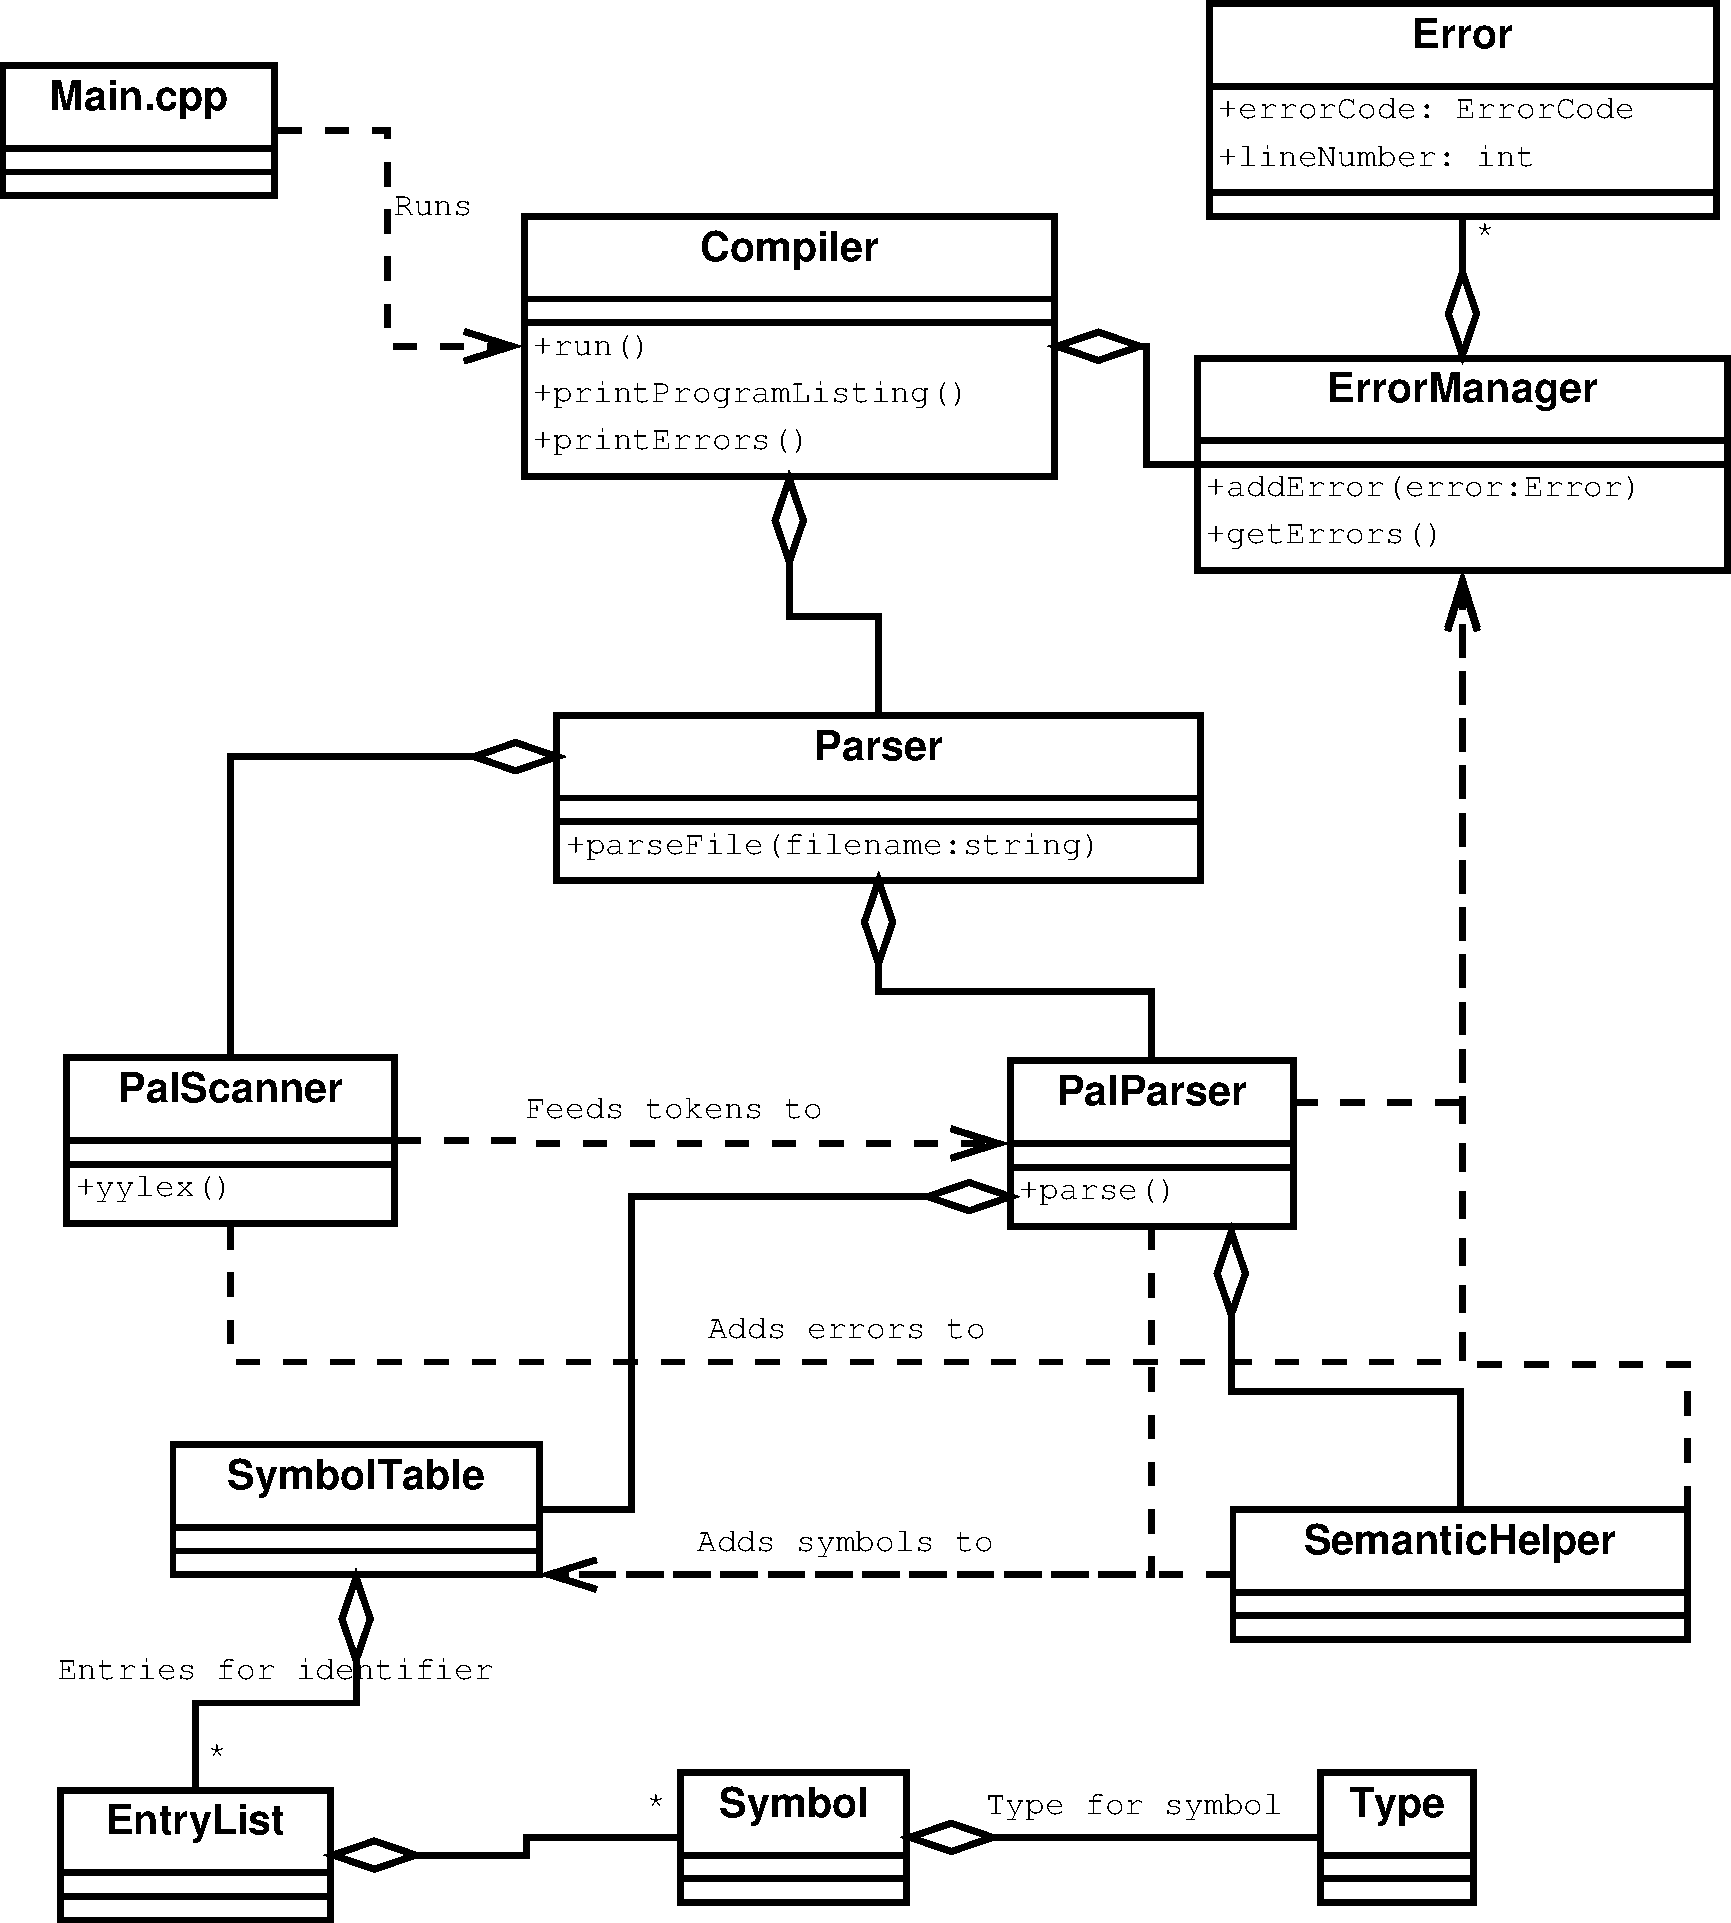
\includegraphics[width=10cm]{uml.pdf}
\caption{General structure of the compiler's parsing components.}
\end{figure}

At this stage, our compiler source consists of 6 classes. The \texttt{Compiler} class is instantiated by 
the program's \texttt{main()} function, and ran with the program's given command line arguments. 

The \texttt{Compiler} class creates an \texttt{ErrorManager}
class which tracks errors as they are detected while parsing the file. It passes the \texttt{ErrorManager}
to the \texttt{Parser} class when it is constructed.

The \texttt{Parser} class is a wrapper for the \texttt{flex} and \texttt{bison}
generated \texttt{PalScanner} and \texttt{PalParser} classes, from the
\texttt{pal.lex} and \texttt{pal.y} sources, respectively. \texttt{Parser}
parses a file with \texttt{parseFile(fileName)}, which creates a
\texttt{PalScanner} and \texttt{PalParser} where the scanner runs through
the file and feeds the parser with a stream of tokens.  The scanner and
parser are given access to the common \texttt{ErrorManager}, and when they
encounter errors during lexical and syntactical analysis, they create new
\texttt{Error} objects with the appropriate error code and line number and
give them to the \texttt{ErrorManager}.

When parsing is finished, the \texttt{Compiler} takes the errors accumulated by the \texttt{ErrorManager}
and either displays them inline with the program listing, or all errors in order of appearance without 
the program listing if \texttt{pal} was invoked with the \texttt{-n} option.

	% Overall design
	% Outline of classes + dependencies

\section*{Lexical Analysis}
	% TODO
	% handling of lexical units
	% syntax error handling at lexical level

\section*{Syntax Analysis}
	% TODO
	% handling of lexical units
	% syntax error reporting
	% recovery strategies

\section*{Testing Strategies}
	% TODO
	% gtest, unit tests
	% whole file tests

% known bugs?
% extra features?

\end{document}
